%%%
% Plantilla de Memoria
% Modificación de una plantilla de Latex de Nicolas Diaz para adaptarla 
% al castellano y a las necesidades de escribir informática y matemáticas.
%
% Editada por: Mario Román
%
% License:
% CC BY-NC-SA 3.0 (http://creativecommons.org/licenses/by-nc-sa/3.0/)
%%%

%%%%%%%%%%%%%%%%%%%%%%%%%%%%%%%%%%%%%%%%%
% Thin Sectioned Essay
% LaTeX Template
% Version 1.0 (3/8/13)
%
% This template has been downloaded from:
% http://www.LaTeXTemplates.com
%
% Original Author:
% Nicolas Diaz (nsdiaz@uc.cl) with extensive modifications by:
% Vel (vel@latextemplates.com)
%
% License:
% CC BY-NC-SA 3.0 (http://creativecommons.org/licenses/by-nc-sa/3.0/)
%
%%%%%%%%%%%%%%%%%%%%%%%%%%%%%%%%%%%%%%%%%

%----------------------------------------------------------------------------------------
%   PAQUETES Y CONFIGURACIÓN DEL DOCUMENTO
%----------------------------------------------------------------------------------------

%%% Configuración del papel.
% microtype: Tipografía.
% mathpazo: Usa la fuente Palatino.
\documentclass[a4paper, 11pt]{article}
\usepackage[protrusion=true,expansion=true]{microtype}
\usepackage{mathpazo}
\usepackage{amsthm}
\usepackage{graphicx}




% Indentación de párrafos para Palatino
\setlength{\parindent}{0pt}
  \parskip=8pt
\linespread{1.05} % Change line spacing here, Palatino benefits from a slight increase by default


%%% Castellano.
% noquoting: Permite uso de comillas no españolas.
% lcroman: Permite la enumeración con numerales romanos en minúscula.
% fontenc: Usa la fuente completa para que pueda copiarse correctamente del pdf.
\usepackage[spanish,es-noquoting,es-lcroman]{babel}
\usepackage[utf8]{inputenc}
\usepackage[T1]{fontenc}
\selectlanguage{spanish}


%%% Gráficos
\usepackage{graphicx} % Required for including pictures
\usepackage{wrapfig} % Allows in-line images
\usepackage[usenames,dvipsnames]{color} % Coloring code


%%% Matemáticas
\usepackage{amsmath}


%%% Bibliografía
\makeatletter
\renewcommand\@biblabel[1]{\textbf{#1.}} % Change the square brackets for each bibliography item from '[1]' to '1.'
\renewcommand{\@listI}{\itemsep=0pt} % Reduce the space between items in the itemize and enumerate environments and the bibliography



%----------------------------------------------------------------------------------------
%   TÍTULO
%----------------------------------------------------------------------------------------
% Configuraciones para el título.
% El título no debe editarse aquí.
\renewcommand{\maketitle}{
  \begin{flushright} % Right align
  
  {\LARGE\@title} % Increase the font size of the title
  
  \vspace{50pt} % Some vertical space between the title and author name
  
  {\large\@author} % Author name
  \\\@date % Date
  \vspace{40pt} % Some vertical space between the author block and abstract
  \end{flushright}
}

%% Título
\title{\textbf{Backtracking II}\\ % Title
Travelling salesman problem} % Subtitle

\author{\textsc{Ignacio Mas Mesa,\\Braulio Valdivielso Martínez} % Author
\\{\textit{Universidad de Granada}}} % Institution

\date{\today} % Date



%----------------------------------------------------------------------------------------
%   DOCUMENTO
%----------------------------------------------------------------------------------------

\begin{document}

\maketitle % Print the title section

%% Resumen (Descomentar para usarlo)
\renewcommand{\abstractname}{Abstract} % Uncomment to change the name of the abstract to something else
\begin{abstract}
En esta ocasión vamos a continuar nuestro estudio de los algoritmos branch and bound, ahora aplicados a uno de los problemas más famosos de las ciencias de la computación: el problema del viajante de comercio (TSP, por sus siglas en inglés). Es la segunda ocasión en la que nos enfrentamos a este problema, pero esta vez buscaremos una solución exacta. Recordaremos que el problema consiste en, dada una lista de ciudades (en nuestro caso puntos en un plano) y una métrica (asumimos la euclídea, pero pueden ser pesos de las aristas de un grafo) encontrar la ruta más corta que pasa exactamente una vez por cada ciudad (volviendo a la de partida). Acabaremos realizando una test de rendimiento de la solución, y comprobaremos que es mucho mejor que otras alternativas exactas.

Este problema ha sido estudiado durante casi cien años desde su planteamiento en 1930, pero sigue siendo interesante en tanto que es un problema NP-hard, i.e., cualquier problema en NP puede ser reducido a él en tiempo polinómico.
\end{abstract}

\vspace{30pt} % Some vertical space between the abstract and first section


%% Índice
  \tableofcontents

\pagebreak

%%% Inicio del documento

\section{Problema}
Nuestro problema es el siguiente:
\begin{quote}
Dada una lista de ciudades (puntos del plano ${\mathbb Q}^2$) encontrar la ruta más corta que pasa exactamente una vez por cada ciudad volviendo a la de partida usando como distancia la euclídea.
\end{quote}

\section{Solución branch and bound}
Sea $M_{i,j}$ la matriz de distancias del mapa que se nos presenta, con $k$ ciudades. Entendemos que el objetivo de nuestro algoritmo es encontrar una permutación $\sigma$ de las $k$ ciudades parar minimizar la siguiente función


$f(\sigma) = \sum\limits_{i=1}^{k} M_{\sigma(i - 1), \sigma(i)}$

El número de permutaciones de $k$ elementos es $k!$, por lo que un algoritmo que comprobara todas sería inviable. Debido a que la cantidad de permutaciones a probar es demasiado grande, se hace necesario conseguir reducir el tamaño de candidatos a probar. Eso lo conseguiremos mediante la poda.

En cada momento nuestro algoritmo tendrá presente una \textbf{cota superior global}, en este caso el coste de la mejor ruta encontrada hasta ahora. Si vemos que una solución parcial que estamos explorando supera este coste, la descartaremos inmediatamente. Más interesantemente, dispondremos de una forma de estimar de forma optimista una \textbf{costa inferior} para cada solución parcial. A partir de estas herramientas podremos establecer que si la estimación del coste de una solución parcial es mayor que la cota superior global, no merece la pena probar la solución.

Además, nuestro algoritmo guardará los candidatos a seguir explorando en una \textbf{cola con prioridad} ordenada según la estimación de cada candidato. De esta manera, los candidatos más prometedores serán explorados antes y además una vez extraigamos de la cola con prioridad un candidato con estimación superior a la cota global, sabremos que todos los que vienen detrás tienen estimación superior, y podremos terminar el algoritmo.

La cota superior será el coste de la mejor solución encontrada hasta el momento. La forma de estimar de forma optimista el coste final de una solución parcial será la siguiente: por cada una de las ciudades que queden por visitar, se encuentra el coste de visitar la ciudad más cercana a esa ciudad. La suma de todos estos costes será una \textbf{estimación por defecto} de la mejor solución que se puede encontrar expandiendo esa solución parcial.


\section{Rendimiento del algoritmo}
Debido a que los sets de datos de la libreria TSPLib eran demasiado grandes para realizar una resolución exacta del problema, tuvimos que generar nuevos sets de datos truncando los anteriores. Comprobamos el correcto funcionamiento de nuestro programa con sets de datos pequeños y comparando nuestros resultados con los de otros compañeros. 

Utilizamos cuatro métricas para medir el rendimiento de nuestra solución:
\begin{itemize}
  \item Número de nodos explorados
  \item Tamaño máximo de la cola con prioridad
  \item Tiempo empleado en resolver el problema
  \item Rutas completas exploradas
\end{itemize}

Los sets de datos que usamos para las siguientes pruebas son distintas versiones del fichero de TSPLib \textit{eil51.tsp} truncados.
 
\subsection{Número de nodos explorados}
\makebox[\textwidth]{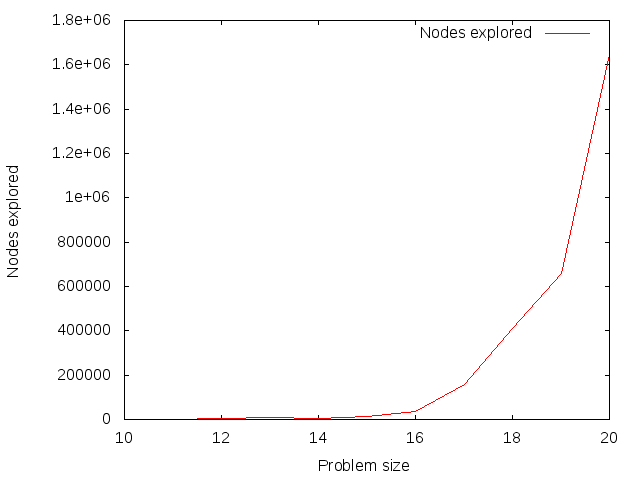
\includegraphics{./results/bbnodes.png}}
Es fácil corroborar el crecimiento explosivo que tiene el número de nodos que se exploran en función del tamaño del problema. Pudiera parecer que esto es necesariamente un fracaso para nuestro algoritmo, pero con una sencilla cuenta podremos comprobar que \textbf{el número de hojas que un algoritmo de fuerza bruta tendría que comprobar es $10^{12}$ veces mayor en el caso con $n = 20$}. Y nos estamos refiriendo exclusivamente al número de hojas, no al de nodos.

\subsection{Tamaño máximo de la cola con prioridad}
\makebox[\textwidth]{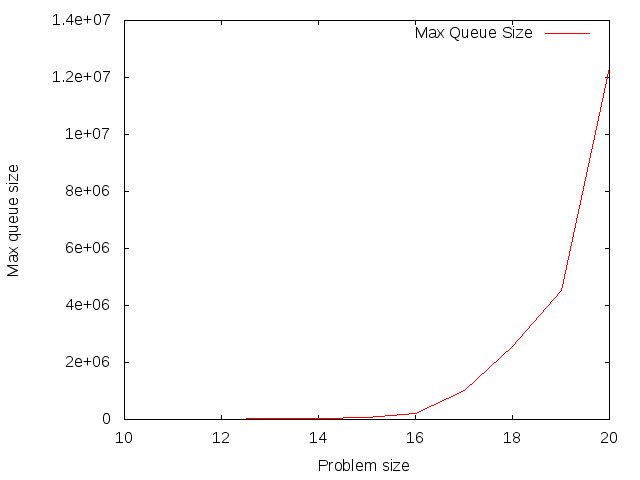
\includegraphics{./results/bbqueuesize.png}}
En este caso el crecimiento también es explosivo. Este gráfico nos muestra que el problema se volverá rápidamente intratable mediante este algoritmo debido a las limitaciones de memoria del computador en el que se ejecute el programa. Esta limitación se puede saltar con el algoritmo \textit{beam search}, que solo se queda con las primeras $k$ entradas de la cola de prioridad, desechando el resto.

\subsection{Tiempo de ejecución}
\makebox[\textwidth]{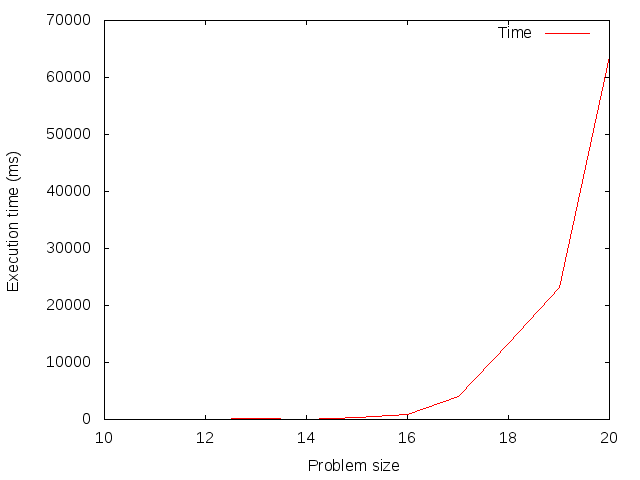
\includegraphics{./results/bbtime.png}}
El tiempo de ejecución se convierte también en un problema en sí mismo. Es esta limitación la que nos ha forzado a no probar el programa para tamaños de problema superiores. En cualquier caso, es muchísimo más rápido que la versión sin branch and bound.

\subsection{Rutas completas exploradas}
\makebox[\textwidth]{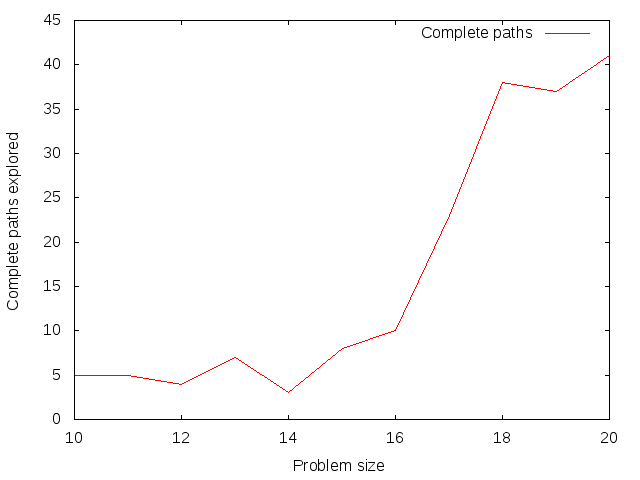
\includegraphics{./results/bbcompletepaths.png}}
La comparación con el número de rutas completas que se pueden trazar en el problema es ridícula.

\section{Conclusiones}
Con esta práctica hemos aprendido cómo funcionan los algoritmos de branch and bound y por qué son la mejor opción para la resolución de cierta clase de problemas. Hemos aprendido cómo utilizando funciones para realizar estimaciones optimistas podemos conseguir descartar un montón de casos que no merece la pena explorar, lo que consigue reducir drásticamente tanto el número de nodos a explorar como el tiempo de ejecución. Asimismo, hemos aprendido que utilizando una cola con prioridad podemos hacer que nuestro algoritmo se encargue de explorar en primer lugar los candidatos más prometedores, resultando en una mejor utilización del tiempo.


\end{document}